\documentclass[12pt]{article}

\usepackage{stoversymb,graphicx,soul}
\usepackage[letterpaper, margin=0.5in, top=0.75in, bottom=1in]{geometry}

\everymath{\displaystyle}

\usepackage{multicol}
\usepackage[many]{tcolorbox}
\usepackage{tikz}

\title{\vspace{-0.75in}\Huge{\red{Exam Review Solutions}}\vspace{-0.5in}}
\date{}

\usepackage[inline]{enumitem}
\setlist[enumerate,1]{leftmargin=0.25in, rightmargin=0.25in,itemsep=7.5mm, topsep=1.5mm}
\setlist[enumerate,2]{leftmargin=0.25in, itemsep=4.5mm}

\newcommand{\shortlim}{\lim_{n\to\infty}}
\newcommand{\sectitle}[1]{\vspace{7.5mm}\noindent\textbf{\Large{#1}}\\[3mm]}
\newcommand{\subsectitle}[2]{\vspace{3mm}\noindent\ul{#1}:\\[3mm]\indent{#2}}
\newcommand{\subsecnoindent}[2]{\vspace{3mm}\noindent\ul{#1}:\\[3mm]{#2}}
\newcommand{\comps}[1]{\left\langle #1_1,#1_2,#1_3\right\rangle}
\newcommand{\compslong}[3]{\left\langle #1, #2, #3\right\rangle}
\newcommand{\pic}[2]{\begin{center}\includegraphics[scale=#1]{#2}\end{center}}
\newcommand{\resultbox}[1]{\begin{center}
		\begin{tcolorbox}[
			enhanced,
			colback=white,
			colframe=black,
			boxrule=0.5pt,
			arc=0pt,
			top=3mm,
			bottom=3mm, 
			width=7in%,
%			grow to left by=0.5in,
			]
			\centering
			#1
		\end{tcolorbox}
\end{center}}
\newcommand{\LH}{L'H\^{o}pital}

\graphicspath{ {./img/} }
\DeclareGraphicsExtensions{.pdf, .png}

\usepackage{caption}
\captionsetup{labelfont=bf, labelformat=simple, justification=centering, labelsep=newline, width=6.5in, textfont={small}}%, textfont={it, footnotesize}}
\captionsetup[figure]{aboveskip=8pt, belowskip=10pt}

\begin{document}
	\maketitle
	
	\red{
	\begin{enumerate}
		\item \begin{enumerate}
			\item $\sqrt{57}$
			\item Does not exist---can't cross a scalar with a vector.
			\item $\compslong{-\frac{3}{17}}{\frac{2}{17}}{-\frac{2}{17}}$
			\item $\compslong{-8}{-11}{1}$
			\item $\sqrt{186}$
			\item Does not exist---can't dot a scalar with a vector.
			\item $\frac{\pi}{2}$
		\end{enumerate}
	
		\item \textbf{Note: }There was a typo in this problem that led to the tangent vector $\vect{r}'(t)$ being the zero vector at $t=0$. For that reason, I told some people to do $t=\pi/4$ for practice. I'm including solutions of both here!
		
		Throughout, note that:
		\begin{itemize}
			\item $\sin(\pi/2-t)=\cos{t}$ and $\cos(\pi/2-t)=\sin{t}$. This isn't necessary to notice, but it makes the derivatives easier \ul{and} these solutions make use of it.
			\item  In light of the above, $\vect{r}'(t)=\compslong{-\sin{t}}{-\sin{t}\cos(\cos{t})}{2t}$.
		\end{itemize}
		
		\ul{t=0}: 
		
		$\vect{r}'(0)=\compslong{0}{0}{0}$ is parallel to the tangent line and $P=\vect{r}(0)=(1,\sin{1},0)$ is on it, so the line is ``point plus vector $t$,'' i.e.
		$$x=1+0t\quad y=\sin{1}+0t\quad z=0+0t\Longrightarrow \boxed{x=1\quad y=\sin{1}\quad z=0}.$$
		
		\ul{$t=\pi/4$}:
		
		$\vect{r}'\left(\frac{\pi}{4}\right)=\compslong{-\frac{1}{\sqrt{2}}}{\frac{\cos\left(\frac{1}{\sqrt{2}}\right)}{\sqrt{2}}}{\frac{\pi}{2}}$ is parallel to the tangent line and $P=\vect{r}\left(\frac{\pi}{4}\right)=\left(\frac{1}{\sqrt{2}},\sin\left(\frac{1}{\sqrt{2}} \right),\frac{\pi^2}{16} \right)$ is on it, so the line (after simplifying) is:
		$$\boxed{x=-\frac{t-1}{\sqrt{2}}\quad y=-\frac{\cos\left(\frac{1}{\sqrt{2}} \right)}{\sqrt{2}}\,t+\sin\left(\frac{1}{\sqrt{2}} \right)\quad z=\frac{1}{16}\pi\left(\pi+8t\right).}$$
		
		\newpage
		
		\item \begin{enumerate}
			\item The plane containing $P$, $Q$, and $R$ necessarily contains the vectors $\vec{PQ}=\compslong{-2}{-4}{2}$ and $\vec{PR}=\compslong{-1}{-5}{-4}$, so the vector $\vec{PQ}\times\vec{PR}$ is perpendicular to it. Therefore,
			$$\vect{n}=\vec{PQ}\times\vec{PR}=\compslong{26}{-10}{6}$$
			is normal to the plane. Using $\vect{n}$ and $P(1,3,5)$, we have the equation of the plane being
			\begin{equation}
				\label{eq:plane}
				\boxed{26(x-1)-10(y-3)+6(z-5)=0}.
			\end{equation}
			\item As in class, we note that the we can parametrize the cylinder $x^2+y^2=4$ using $x=2\cos{t}$ and $y=2\sin{t}$. Plugging these into \eqref{eq:plane} and solving for $z$ yields
			$$z=\frac{1}{3} (10 \sin{t}-26 \cos{t}+13),$$
			and so the parametrization of this curve is
			$$\boxed{\vect{r}(t)=\compslong{2\cos{t}}{2\sin{t}}{\frac{1}{3} (10\sin{t}-26\cos{t}+13)}}.$$
			
			This curve can be seen below.
			
			\begin{center}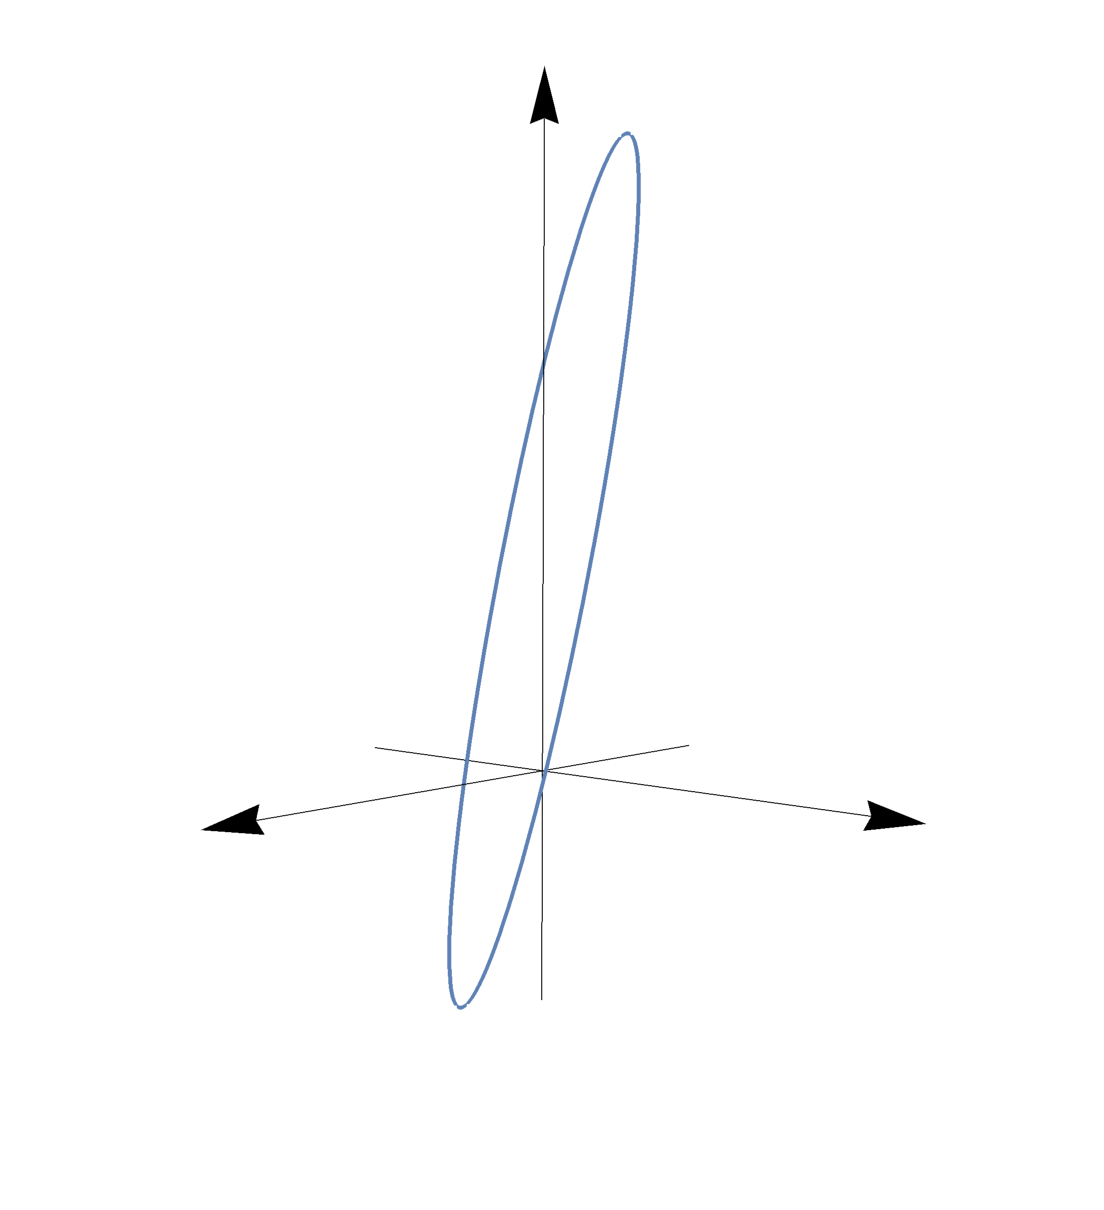
\includegraphics[scale=0.7]{ExamReviewAnswerCurve}\end{center}
			\end{enumerate}
		
			\newpage
			
			\item Note that after simplification,
			$$\vect{r}'(t)=\compslong{e^t\cos{t}-e^t\sin{t}}{e^t}{e^t\sin{t}+e^t\cos{t}}$$
			and
			$$\vect{r}''(t)=\compslong{-2 e^t \sin{t}}{e^t}{2e^t\cos{t}}.$$
			
			\begin{enumerate}
				\item $\Reals$
				\item Velocity is $\vect{r}'(t)=\compslong{e^t\cos{t}-e^t\sin{t}}{e^t}{e^t\sin{t}+e^t\cos{t}}$\\[3mm]
				Speed is $|\text{velocity}|=|\vect{r}'(t)|=\sqrt{3}e^t$\\[3mm]
				Acceleration is $\vect{r}''(t)=\compslong{-2 e^t \sin{t}}{e^t}{2e^t\cos{t}}$.
				\item $\vect{T}(t)=\compslong{\frac{\cos{t}-\sin{t}}{\sqrt{3}}}{\frac{1}{\sqrt{3}}}{\frac{\sin{t}+\cos{t}}{\sqrt{3}}}$
				\item $\vect{N}(t)=\compslong{-\frac{\sin{t}+\cos{t}}{\sqrt{2}}}{0}{\frac{\cos{t}-\sin{t}}{\sqrt{2}}}$
				\item $\vect{B}(t)=\vect{T}(t)\times\vect{N}(t)=\compslong{\frac{\cos{t}-\sin{t}}{\sqrt{6}}}{\sqrt{\frac{2}{3}}}{\frac{\sin{t}+\cos{t}}{\sqrt{6}}}$
				\item $\kappa(t)=\frac{\sqrt{2}}{3}e^{-t}$
				\item $a_T=\sqrt{3} e^t$
				\item $a_N=\sqrt{2} e^t$\\
				
				\textbf{Note: }Simplifying $a_T\vect{T}+a_N\vect{N}$ yields
				$$a_T\vect{T}+a_N\vect{N}=\compslong{-2 e^t \sin{t}}{e^t}{2e^t\cos{t}}=\vect{a}(t),$$
				as expected (because, remember: $\vect{a}(t)$ \textit{should} equal $a_T\vect{T}+a_N\vect{N}$ for all $t$...).
			\end{enumerate}
		

%			\item The curvature $\kappa(t)$ of $\vect{r}$
%			\item The tangential component of the acceleration $\vect{a}(t)$
%			\item The normal component of $\vect{a}(t)$
%		\end{enumerate}
	\end{enumerate} }
\end{document}